% Vorgaben Assignment aus Studienheft SQL03
% Formatvorgaben fuer den Text
% Umfang: 8 - 10 Seiten (inkl. Abbildungen und Tabellen, aber ohne Deckblatt, % Gliederung und Literaturverzeichnis, Eidesstattliche Erklaerung)
% Zeilenabstand: 1,5
% Schriftart: frei
% Schriftgrad: 12 pt
% Variablen, physikalische Groessen und Funktionszeichen werden kursiv gedruckt.
% Korrekturrand: links: 4,5 cm, rechts 2,0 cm, oben und unten jeweils 3,0 cm
% Deckblatt: (Adresse, AKAD-E-Mail-Adresse, Immatrikulationsnummer, Modul-
% bezeichnung, Thema, Datum, Felder für Korrektor)
% Gliederung (1 Seite)
% Literaturverzeichnis (3 - 5 Literaturquellen  z. B. Lehrbuecher, aktuelle Fachartikel recherchieren)
% Eidesstattliche Erklaerung (unterschrieben und fest eingebunden)
% Bearbeitungsdauer: 2 Monate


\documentclass[a4paper,12pt]{article}
\usepackage[ngerman]{babel}
\usepackage[nottoc]{tocbibind} % Anzeigen des Literaturverzeichnisses im TOC
\usepackage{epsfig}
\usepackage{times}
\usepackage{supertabular}
\usepackage{wrapfig}
\usepackage{multirow}
\usepackage[onehalfspacing]{setspace}
\usepackage{listings}
\usepackage{mathptmx}
\usepackage{geometry}
\usepackage{helvet}
\usepackage{courier}
\usepackage{setspace}
\usepackage{textcomp}
\usepackage[T1]{fontenc}
\usepackage[utf8]{inputenc}
\usepackage{fancyhdr}
\usepackage{float} % Notwendig fuer figure[h]
\usepackage[printonlyused]{acronym}

\newif\iflistoffigures
\newif\iflistoftables
\newif\ifacronym

%Titel
\newcommand*{\Titel}{} 

%Betreff
\newcommand*{\Betreff}{Assignment im Modul ABC01 - \\ Vorlage \LaTeX{}} 

%Betreuer
\newcommand*{\Betreuer}{Betreuer: Prof. Franz--Karl Schmatzer} 

%Vor- und Nachname
\newcommand*{\Name}{Stefan Waidele}

%Straße und Hausnummer
\newcommand*{\Strasse}{Ensisheimer Straße 2} 

%Plz und Ort
\newcommand*{\PlzOrt}{79395 Neuenburg am Rhein} 

%Immatrikulationsnummer
\newcommand*{\Immatrikulationsnummer}{102 81 71}

%Email 
\newcommand*{\Email}{Stefan.Waidele@AKAD.de} 


% Verzeichnisse (Wenn nicht benötigt, Zeile mit % auskommentieren oder löschen

%% Abbildungsverzeichnis 
\listoffigurestrue
%% Tabellenverzeichnis
%\listoftablestrue
%% Abkürzungsverzeichnis
%\acronymtrue


% Wittwen und Waisen verhindern
\clubpenalty10000
\widowpenalty10000
\displaywidowpenalty=10000

\usepackage[flushmargin,hang,ragged]{footmisc}
\usepackage{lmodern} %Type1-Schriftart für nicht-englische Texte
\usepackage{fancyhdr}

\usepackage[
	pdftitle={\Titel},
	pdfsubject={Datenbankgestützte PHP--Anwendung für eine Umfrage--Website},
	pdfauthor={Stefan Waidele},
	pdfkeywords={akad, dba02, assignment, wirtschaftsinformatik}
	hyperfootnotes=false,
	colorlinks=true,
	linkcolor=black,
	urlcolor=black,
	citecolor=black
]{hyperref}

%\renewcommand{\familydefault}{\rmdefault}
\renewcommand{\bflabel}[1]{\normalfont{\normalsize{#1}}\hfill}

%% Definition for Codeschnipsel im Fließtext
\newcommand{\code}{\texttt}

%% Für Codeblöcke mit Syntax-Highlighting
%% http://www.ctan.org/tex-archive/macros/latex/contrib/minted/
\usepackage{minted}
\definecolor{bg}{rgb}{0.95,0.95,0.95}


\makeatother

\geometry{a4paper, left=45mm, right=20mm, top=30mm, bottom=30mm}
\pagenumbering{roman}

\begin{document}
	
\parskip=1em
\parindent=0cm

%description: Deckblatt in Deutsch
%% Basierend auf einer TeXnicCenter-Vorlage von Tino Weinkauf.
%% sowie der akad-vorlage von Daniel Falkner
%%%%%%%%%%%%%%%%%%%%%%%%%%%%%%%%%%%%%%%%%%%%%%%%%%%%%%%%%%%%%%

%%%%%%%%%%%%%%%%%%%%%%%%%%%%%%%%%%%%%%%%%%%%%%%%%%%%%%%%%%%%%
%% Deckblatt
%%%%%%%%%%%%%%%%%%%%%%%%%%%%%%%%%%%%%%%%%%%%%%%%%%%%%%%%%%%%%
%%
%% ACHTUNG: Sie benötigen ein Hauptdokument, um diese Datei
%%          benutzen zu können. Verwenden Sie im Hauptdokument
%%          den Befehl "\input{dateiname}", um diese
%%          Datei einzubinden.
%%

\begin{titlepage}

%\thispagestyle{empty}

\vspace{5cm}

\Name \\ 
\Strasse \\ 
\PlzOrt\\ 
\href{mailto:\Email}{\Email}

AKAD Hochschule Stuttgart\\
Immatrikulationsnummer: \Immatrikulationsnummer

\vfill

\begin{tabbing}
Modul DBA02 --- \=Praktisches Arbeiten mit Datenbanken\\ 
                \>Assignment  
\end{tabbing}
\LARGE
\textsc{Datenbankgestützte \\PHP--Anwendung\\für eine Umfrage-Website}\\

\vfill

\normalsize

Betreuer: Prof. Dr. Franz--Karl Schmatzer

\today %%Datum der Abgabe - am besten selbst reinschreiben.

\vfill


\includegraphics[width=3cm]{akad_logo.png}

AKAD Hochschule Stuttgart

\end{titlepage}


%
\includegraphics[scale=0.35]{akad_logo.png}

%\clearpage
\normalsize


\normalsize

\begin{spacing}{1.0} % Verzeichnisse werden mit einzeiligem Abstand gesetzt
\parskip=0em
\newpage

% Inhaltsverzeichnis
\tableofcontents 
\newpage

% Abbildungsverzeichnis
\iflistoffigures
\listoffigures 
\newpage
\fi

% Tabellenverzeichnis
\iflistoftables
\listoftables 
\newpage
\fi

% Abkürzungsverzeichnis
\ifacronym
\section*{Abkürzungsverzeichnis}
\addcontentsline{toc}{section}{Abkürzungsverzeichnis} 
\begin{acronym}[ABK]
	\acro{Abk}{Abkürzungen}
	\acro{Test}{Wird nicht im Text verwendet und taucht auch nicht im Verzeichnis auf}
\end{acronym}

\fi

\parskip=1em
\end{spacing} 

\clearpage

\newcounter{romanPagenumber} 
\setcounter{romanPagenumber}{\value{page}} % Roemische Seitenanzahl speichern.


\pagestyle{fancy}
\fancyhead{}
\fancyhead[LO,RE]{\textsc{\Titel}}
\fancyhead[RO,LE]{\thepage}
\fancyfoot[CO,CE]{}

\nocite{*} 

\pagenumbering{arabic}

\begin{spacing}{1.5} % Zeilenabstand: 1,5 fuer den Textteil

\section{Einleitung}
\subsection{Aufgabenstellung}

Im Rahmen des Moduls DBA02 war eine datenbankgestützte PHP--Anwendung für eine Website zu erstellen, welche die folgenden Kriterien erfüllt:

\begin{itemize}
\item \textbf{Frage stellen}: Besuchern der Website soll eine Frage gestellt werden, auf die sie mit einer oder mehreren vorgegebenen Möglichkeiten antworten können.
\item \textbf{Auswertung}: Nach der Beantwortung der Frage soll dem Besucher eine Auswertung der bisher gegebenen Antworten (Angaben in Prozent) gezeigt werden.
\item \textbf{Benutzerverwaltung}: Ein Administrator soll sich bei der Anwendung anmelden können. Hierzu soll ein Benutzername und Passwort abgefragt und geprüft werden.
\item \textbf{Neue Fragen eingeben}: Dem Seitenadministrator soll es über ein Formular möglich sein, neue Fragen mit den zugehörigen Antwortmöglichkeiten einzugeben. Normalen Besucher der Website ist diese Möglichkeit zu verwehren.  
\item \textbf{Datenbank}: Alle benötigten Daten werden in einer MySQL--Datenbank gespeichert.
\item \textbf{Echtzeitstatistiken}: Die Auswertung der gegebenen Antworten soll unmittelbar vor der Anzeige berechnet werden.
\item \textbf{XAMP}: Die Anwendung soll mit der Kombination von Apache--Webserver, MySQL--Datenbank und PHP als Programiersprache lauffähig sein. Das Betriebssystem kann frei gewählt werden. 
\end{itemize}

Desweiteren sollte die Anwendung objektorientiert programmiert werden, Enturfsmuster verwenden und die HTML--Ausgabe per CSS formtiert werden.

\subsection{Gemeinschaftsarbeit}

Die Aufgabe war arbeitsteilig in Teamarbeit zu lösen. Das der Anwendung zu Grunde liegende Datenmodell wurde gemeinsam in einer Teambesprechung erarbeitet und festgelegt. Anschließend wurde ein Mockup\footnote{engl. für Attrappe. (to mock: nachahmen)} der HTML--Seiten und die benötigten SQL--Abfragen, gefolgt von einem prozedural programmierten Prototypen erstellt. Hierbei erstellte der Autor die für die Benutzerverwaltung und Frageneingabe notwendige Programmteile. Die Abfrage-- und Auswertungsseiten wurden von Yvonne Frezel gefertigt.

Da die im Seminar DBA02 begonnene Umsetzung des Programmcodes in Klassen unterschiedliche Richtungen verfolgte, wurde die enge Teamarbeit anschließend nicht mehr weitergeführt. Aufgrund der gemeinsamen Datenbasis sind die vom Author und von Frenzel erstellten PHP--Dateien miteinander kombinierbar, auch wenn sie intern andere Klassen und Zugriffsmethoden nutzen.

Dieses Assignment geht hauptsächlich auf die vom Autor konzipierten Programmteile „Benutzerverwaltung“ und „Neue Fragen hinzufügen“ ein.

\subsection{Aufbau der Arbeit}

Zunächst werden im Grundlagenkapitel \ref{sec:grundlagen} die verwendeten Konzepte, Schnittstellen und Frameworks beschrieben. Anschließend wird das Datenbankschema im Kapitel \ref{sec:dbschema} und die erstellte PHP--Klassenhierarchie in Kapitel \ref{sec:klassen} ausführlich dargestellt. Erläuterungen zur darauf aufbauenden Implementierung der Anwendung mit Hilfe von PHP und HTML schließen in Kapitel \ref{sec:anwendung} den Hauptteil dieser Arbeit ab.

\subsection{Abgrenzung}

Da eine datenbankgestützte Web--Anwendung in der Regel einem großen Personenkreis\footnote{allen Internet-- oder zumindest Intranetnutzern} zur Verfügung steht sind hier unbedingt Sicherheitsaspekte zu beachten. Da eine ausführliche Betrachtung dieser Maßnahmen den Rahmen dieses Dokuments sprechengen würde, werden nur entsprechende Hinweise auf weiterführende Informationen gegeben. Auch Performance--Überlegungen gehen nur in sehr beschränktem Maß in die Implementation ein.



\section{Grundlagen}
\label{sec:grundlagen}
\subsection{Entwurfsmuster: Fassade}

Beim Fassaden--Entwurfsmuster gewährt eine Klasse einen einfachen Zugriff auf ein beliebig komplexes System weiterer Klassen. Der Nutzer der Fassadenklasse benötigt kein Wissen über die Funktionsweise der Klassenhierarchie hinter der Fassade, kann jedoch auf diese zugreifen, falls die bereitgestellte Funktionalität nicht ausreicht\footnote{vgl. \cite{Balzert}, Seite 367ff}.

In der hier erstellten Anwendung wird der Zugriff auf die Datenbank über die Fassaden--Klasse \code{SQL} realisiert. Diese erstellt das Low--Level Objekt der Klasse \code{Datenbank}, bereitet die notwendigen SQL--Abfragen vor und gibt die Resultate dann als String oder als Array von Strings zurück. Die aufrufenden Routinen benötigen kein Wissen über die verwendete Datenbankschnittstelle oder über die Details der Abfragen. Sollten die in der Klassendefinition vorgesehenen Abfragen allerdings nicht ausreichen, kann auch direkt auf die Klasse \code{Datenbank} zugegriffen werden.

\subsection{Entwurfsmuster: Singleton}

Das Klasse nach dem Singleton--Entwurfsmuster stellt sicher, dass sie in einem Programm nur ein einziges Mal instanziiert wird. Allen Nutzern der Klasse wird dann eine Referenz auf ebendiese Instanz übergeben. Der Zugriff erfolgt jeweils auf die gleichen Daten, die somit global zur Verfügung gestellt werden\footnote{vgl. \cite{Balzert}, Seite 361ff}.

Somit bildet das Singleton--Entwurfsmuster eine passende Grundlage für die Nutzerverwaltung, da immer nur ein Benutzer angemeldet sein kann\footnote{Dies gilt jeweils pro Browser--Instanz. In einem weiteren Browserfenster mit eigenen Cookies kann sich ein weiterer Nutzer anmelden, jedoch auch wieder nur einer}.

Das Singleton-Entwurfsmuster kann aufgrund seiner Eigenschaften als objektorientierte Umsetzung von globalen Variablen mit all deren Vor-- und Nachteilen gesehen werden und wird daher auch als „Anti--Pattern“ kritisiert\footnote{vgl. \cite{Hauer:singleton}}.

\subsection{PHP--Schnittstelle: Session--Cookies}

Da HTTP ein zustandsloses Protokoll ist, wird ein Mechanismus benötigt, mit dem gespeichert werden kann, ob es sich beim Besucher der Website um einen angemeldeten Benutzer handelt oder nicht. Die von PHP bereitgestellten Session--Cookies können eine begrenzte Menge Daten (ca. 4kB), die im Browser gespeichert wird, von Seitenaufruf zu Seitenaufruf weitergeben werden\footnote{vgl. \cite{Theis}, S. 417ff}.

Die hier besprochene Anwendung verwendet diese Möglichkeit um den Anmeldestatus (\code{angemeldet==TRUE} bzw. \code{angemeldet==FALSE}) und den Benutzernamen zu speichern.

\subsection{PHP--Schnittstelle: PDO}

Der Datenbankzugriff wird in der beschriebenen Anwendung über die PDO--Klasse\footnote{PDO: PHP Data Object} realisiert. Diese sorgt für den Verbindungsaufbau zur MySQL--Datenbank und stellt Schutzmechanismen gegen SQL--Injection Angriffe bereit. Für einen solchen Angriff müssen die Benutzereingaben ungeprüft in die SQL--Abfrage (z.B. durch einfache Variablen--Substitution) übernommen werden. Diese wird dadurch dann so verändert, dass sensible Daten ausgespäht oder die Daten verändert bzw. gelöscht werden können\footnote{vgl. \cite{friedl:sqlinjection}}. Die Überprüfung der Eingabewerte ist somit in jedem Falle empfehlenswert und aufgrund des öffentlichen Charakters der Webanwendung hier besonders wichtig.

\subsection{HTML--Designframework: Bootstrap}

Die hier vorgestellte Anwendung realisiert ihr Aussehen zum großen Teil mit dem CSS--Framework „Bootstrap“, welches moderne Designprinzipien wie variables, mehrspaltiges Layout oder gar responsives Layout, welches sich an die unterschiedlichen Bildschirmgrößen vom Smartphone bis zum wandfüllenden HD--TV anpassen kann, anbietet\footnote{Lizenz: Apache Licence V2.0, Download unter \url{http://getbootstrap.com/}}.

Die Anwendung selbst muss den entsprechenden Elementen lediglich die gewünschten CSS--Klassen zuweisen. Der Entwickler wird somit nicht mit den Design--Details belastet.

Trotz allem ist eine eigene Anpassung des Designs wie in der Datei \code{…/style.css} zu sehen ist, möglich. 

\subsection{JavaScript--Frontendramework: jQuery}

Bei der Realisierung der Eingabeseite für neue Fragen und Antwortmöglichkeiten wird die JavaScript Bibliothek „jQuery“ verwendet, um weitere Antwortmöglichkeiten einfügen oder diese auch wieder löschen zu können. jQuery bietet auch noch weitere Funktionen für interaktive Benutzeroberflächen, die allerdings in der hier beschriebenen Anwendung nicht genutzt werden.\footnote{Lizenz: MIT-Licence, Download unter \url{http://jquery.com/}}




\section{Datenbank--Schema}

\subsection{Konzeptuelles Datenbankschema: Entity--Relationship Diagram}

Hier werden die Gegenstände der realen Welt modelliert wie in Abbildung \ref{fig:erd} gezeigt modelliert. Hierbei ist zu beachten, dass die Entität „Frage“ das zentrale Element des Datenmodells darstellt. Die weiteren Entitäten „Antwortmöglichkeit“ bzw. „gegebene Antwort” sind existenzabhängige Entities. Ohne Antwortmöglichkeit kann ohne zugehörige Frage nicht existieren, eine gegebene Antwort macht nur Sinn, wenn es eine entsprechende Antwortmöglichkeit und Frage gibt.

Die Entität „Benutzer“ steht in keiner Beziehung zu den anderen Entitäten, sie wird auch nur für die Eingabe neuer Fragen und Antwortmöglichkeiten, bzw. zur Authentifizierung benötigt.

\begin{figure}[H]
\begin{center}
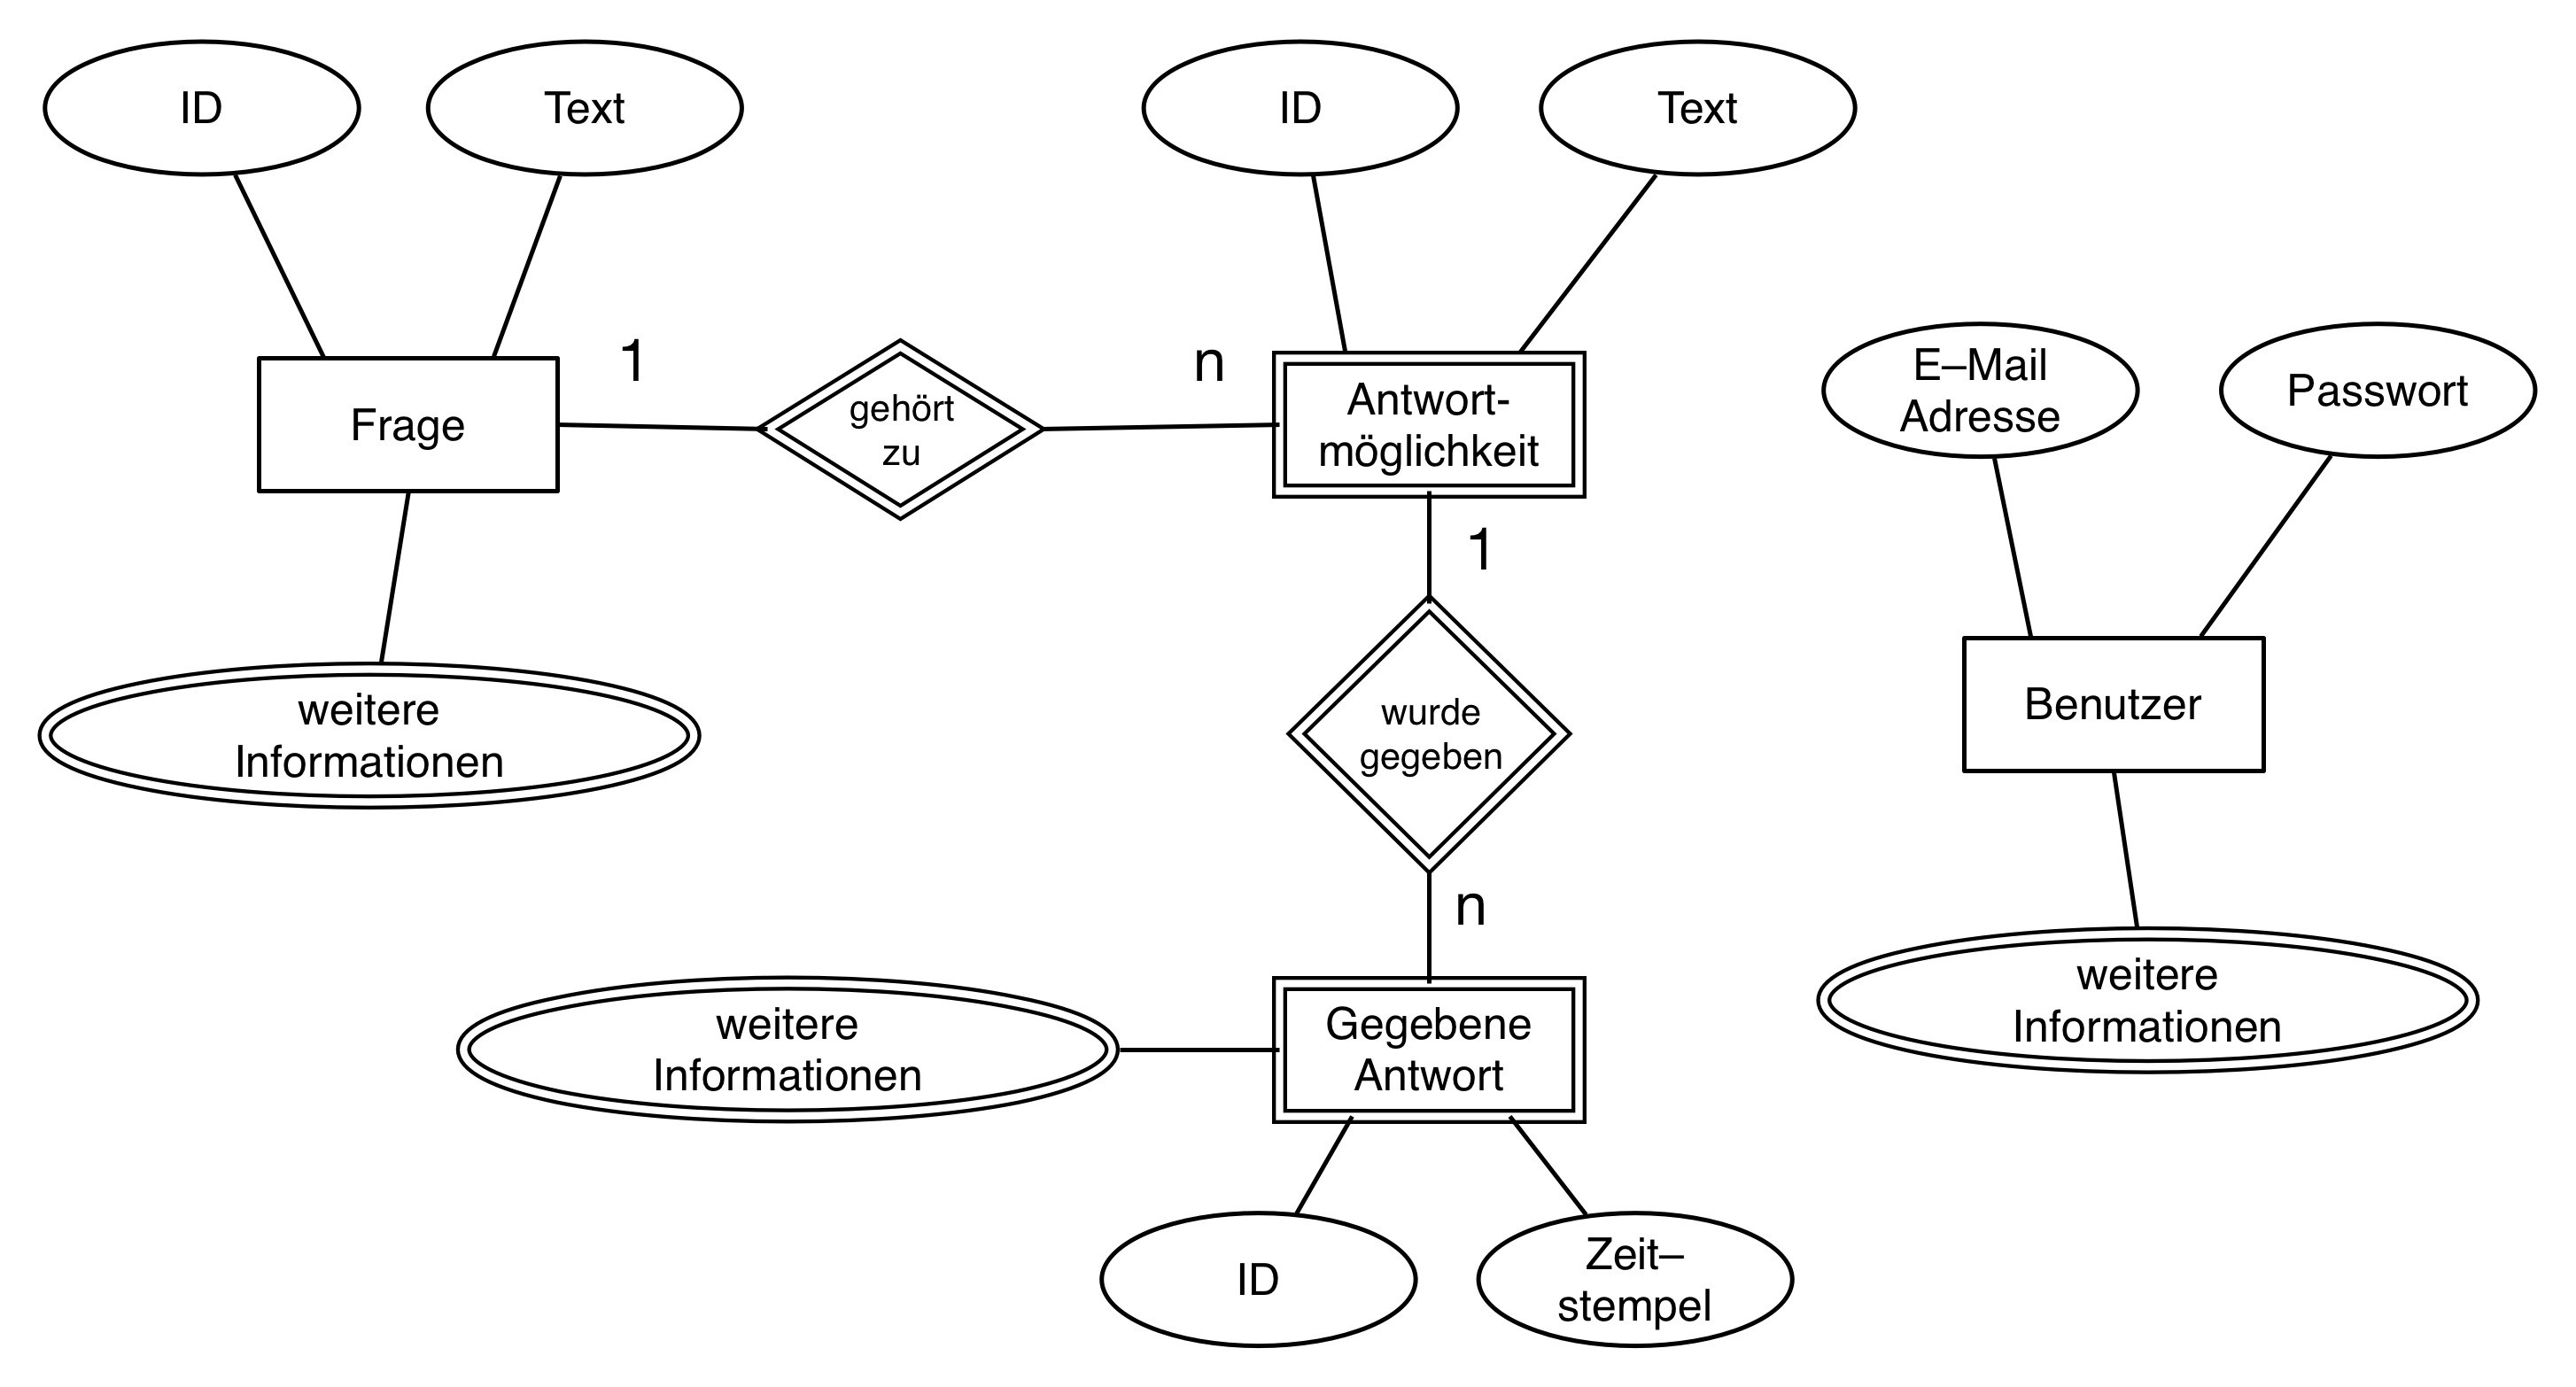
\includegraphics[width=\textwidth]{ERD.jpg}
\caption{Entity Relationship Diagram}
\end{center}
\label{fig:erd}
\end{figure}

Die als zsammengesetzte Attribute dargestellten „weiteren Informationen“ sind Attribute der jeweiligen Entitäten, die für die gestellten Anforderungen nicht notwendig sind, jedoch im Produktivbetrieb großen Zusatznutzen bieten könnten. So wäre es möglich die gegebenen Antworten durch die Speicherung der IP--Adresse, Browser--Fingerprinting\footnote{Die Identifikation eines speziellen Nutzers durch Konfigurationsdetails des Webbrowsers, Bildschirmgröße, Betriebssystemversion, etc. Siehe auch \url{https://panopticlick.eff.org/}} oder andere Techniken genauer zu identifizieren und somit einem bestimmten Nutzer zuzuordnen. Hierbei sind dann die jeweiligen Datenschutzbestimmungen zu beachten.

Die Datensätze der Entity „Frage“ könnten Zeitangaben enthalten, die festlegen wann bzw. wie lange eine Frage auf der Website angezeigt wird. Die Antwortmöglichkeiten könnten durch entsprechende Angaben zur Sortierreihenfolge geordnet werden.

\subsection{Logisches Datenbankschema: Entity--Relationship Diagram}

Aufgrund des in Abbildung \ref{fig:erd} auf Seite \pageref{fig:erd} dargestelten Modell ergibt sich folgende Relationen:


\subsection{Tabelle: user}
\begin{center}
\tablehead{ \textbf{user} & & 
\\ }
\bottomcaption[Beschreibung]{Beschreibung. Quelle: Berger, Vorlesung, 2012, München }
\begin{supertabular}{c|c|c}
\hline
email & varchar(255) &  \\
pw & char(32) &  \\
\end{supertabular}
\end{center}


\begin{figure}[h]
\begin{minted}[bgcolor=bg]{sql}
CREATE TABLE user (
  email VARCHAR(255) NOT NULL,
  pw CHAR(32) NOT NULL,
  create_time TIMESTAMP DEFAULT CURRENT_TIMESTAMP,
  PRIMARY KEY (`email`));
\end{minted}
\caption{SQL: CREATE TABLE user}
\label{sql:tbluser}
\end{figure}

Als Benutzername wird hierbei die E--Mail Adresse des Administrators genutzt. 

Das Passwort sollte nicht im Klartext in der Datenbank gespeichert werden. Ein \code{salted hash}\footnote{Also der Hashwert des Passworts, welches zuvor mit Applikationsspezifischen Zusatzdaten ergänzt wurde} schützt hier das Passwort vor dem Ausspähen durch den Administrator selbst\footnote{Seit Vodafone 2013 eine dokumentierte Gefahr} oder durch Angreifer.\\
Die hier reservierten 32 Byte sind für den in der MySQL--Dokumentation\footnote{\cite{mysql-pcrypt}} emphohlenen MD5-Hash ausreichend. Da die entsprechende PHP--Dokumentation\footnote{\cite{php-pcrypt}} hier allerdings eine genau entgegengesetzte Empfehlung gibt, ist dieser Sicherheitsaspekt für ein Produktivsystem nochmals genauer zu prüfen.

\subsection{Tabelle: frage}
\begin{figure}[h]
\begin{minted}[bgcolor=bg]{sql}
CREATE TABLE frage (
  fid INT NOT NULL AUTO_INCREMENT,
  txt VARCHAR(1024) NOT NULL,
  PRIMARY KEY (`fid`));
\end{minted}
\caption{SQL: CREATE TABLE frage}
\label{sql:tblfrage}
\end{figure}

\subsection{Tabelle: antwort}
\begin{figure}[h]
\begin{minted}[bgcolor=bg]{sql}
CREATE TABLE antwort (
  aid INT NOT NULL AUTO_INCREMENT,
  nr  INT NULL,
  txt VARCHAR(1024) NOT NULL,
  fid INT NOT NULL,
  PRIMARY KEY (`aid`),
  FOREIGN KEY (`fid`) REFERENCES frage(`fid`));
\end{minted}
\caption{SQL: CREATE TABLE antwort}
\label{sql:tblantwort}
\end{figure}

\subsection{Tabelle: geantwortet}
\begin{figure}[h]
\begin{minted}[bgcolor=bg]{sql}
CREATE TABLE geantwortet (
  gid INT NOT NULL AUTO_INCREMENT,
  aid INT NOT NULL,
  zs TIMESTAMP DEFAULT CURRENT_TIMESTAMP,
  PRIMARY KEY (`gid`),
  FOREIGN KEY (`aid`) REFERENCES antwort(`aid`));
\end{minted}
\caption{SQL: CREATE TABLE geantwortet}
\label{sql:tblgeantwortet}
\end{figure}

\subsection{Query: Frage -- Text}
Wird für die Abfrage und Auswertung benötigt.

\begin{figure}[h]
\begin{minted}[bgcolor=bg]{sql}
select txt from frage where fid = <n>;
\end{minted}
\caption{SQL: Text von Frage <n>}
\label{sql:qfragetxt}
\end{figure}

\subsection{Query: Antwortmöglichkeiten}
Wird für die Abfrage benötigt.

\begin{figure}[h]
\begin{minted}[bgcolor=bg]{sql}
select antwort.txt
	from antwort
	where fid = <n> 
\end{minted}
\caption{SQL: Mögliche Antworten für Frage <n>}
\label{sql:qantwnum}
\end{figure}


\subsection{Query: Anzahl der gegebenen Antworten}
Wird für die Auswertung benötigt: 100\%

\begin{figure}[h]
\begin{minted}[bgcolor=bg]{sql}
select count(geantwortet.aid) 
	from antwort, geantwortet 
	where geantwortet.aid = antwort.aid and antwort.fid = <n>;
\end{minted}
\caption{SQL: Antwortzahl 100\% von Frage <n>}
\label{sql:qantw100}
\end{figure}

\subsection{Query: Gegebene Antworten und Häufigkeit}
Wird für die Auswertung benötigt.

\begin{figure}[h]
\begin{minted}[bgcolor=bg]{sql}
select antwort.txt, count(geantwortet.aid) 
	from antwort, geantwortet 
	where geantwortet.aid = antwort.aid and antwort.fid = <n> 
	group by geantwortet.aid;
\end{minted}
\caption{SQL: Gegebene Antworten mit Häufigkeit für Frage <n>}
\label{sql:qantwnum}
\end{figure}




\subsection{Tabelle}

\begin{center}
\tablehead{ \textbf{Head1} & \textbf{Head2} & \textbf{Head3}
\\ }
\bottomcaption[Beschreibung]{Beschreibung. Quelle: Berger, Vorlesung, 2012, München }
\begin{supertabular}{c|c|c}
\hline
1 & 2 & 3 \\
4 & 5 & 6 \\
7 & 8 & 9 \\
1 & 2 & 3 \\
4 & 5 & 6 \\
7 & 8 & 9 \\
\end{supertabular}
\end{center}

\subsection{Bilder}

\begin{figure}[H]
\begin{center}
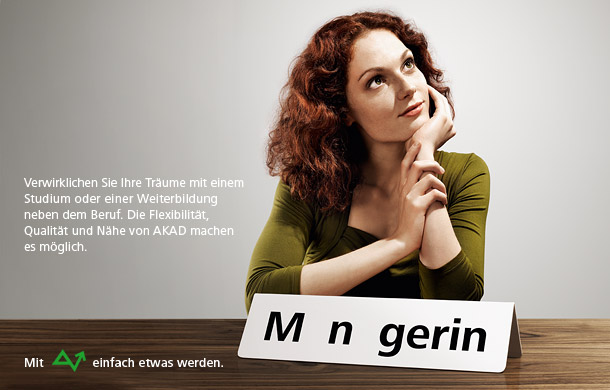
\includegraphics[scale=0.5]{akad_bild1.jpg}
\caption[Akad]{Akad. Quelle: www.akad.de}
\end{center}
\end{figure}

\subsection{Syntax Highlighting}
\begin{figure}[h]
\begin{minted}[bgcolor=bg]{php}
<?php 
$title="Lorem";
$desc = "Lorem Ipsum";
include($_SERVER['DOCUMENT_ROOT'].'/header.php'); 
?>
\end{minted}
\caption{Quellcode: Aufruf von header.php (PHP)}
\label{abb:header}
\end{figure}

\section{Datenbank--Schema}

\subsection{Konzeptuelles Datenbankschema: Entity--Relationship Diagramm}

Hier werden die Gegenstände der realen Welt modelliert wie in Abbildung \ref{fig:erd} gezeigt modelliert. Hierbei ist zu beachten, dass die Entität „Frage“ das zentrale Element des Datenmodells darstellt. Die weiteren Entitäten „Antwortmöglichkeit“ bzw. „gegebene Antwort” sind existenzabhängige Entities. Ohne Antwortmöglichkeit kann ohne zugehörige Frage nicht existieren, eine gegebene Antwort macht nur Sinn, wenn es eine entsprechende Antwortmöglichkeit und Frage gibt.

Die Entität „Benutzer“ steht in keiner Beziehung zu den anderen Entitäten, sie wird auch nur für die Eingabe neuer Fragen und Antwortmöglichkeiten, bzw. zur Authentifizierung benötigt.

\begin{figure}[H]
\begin{center}
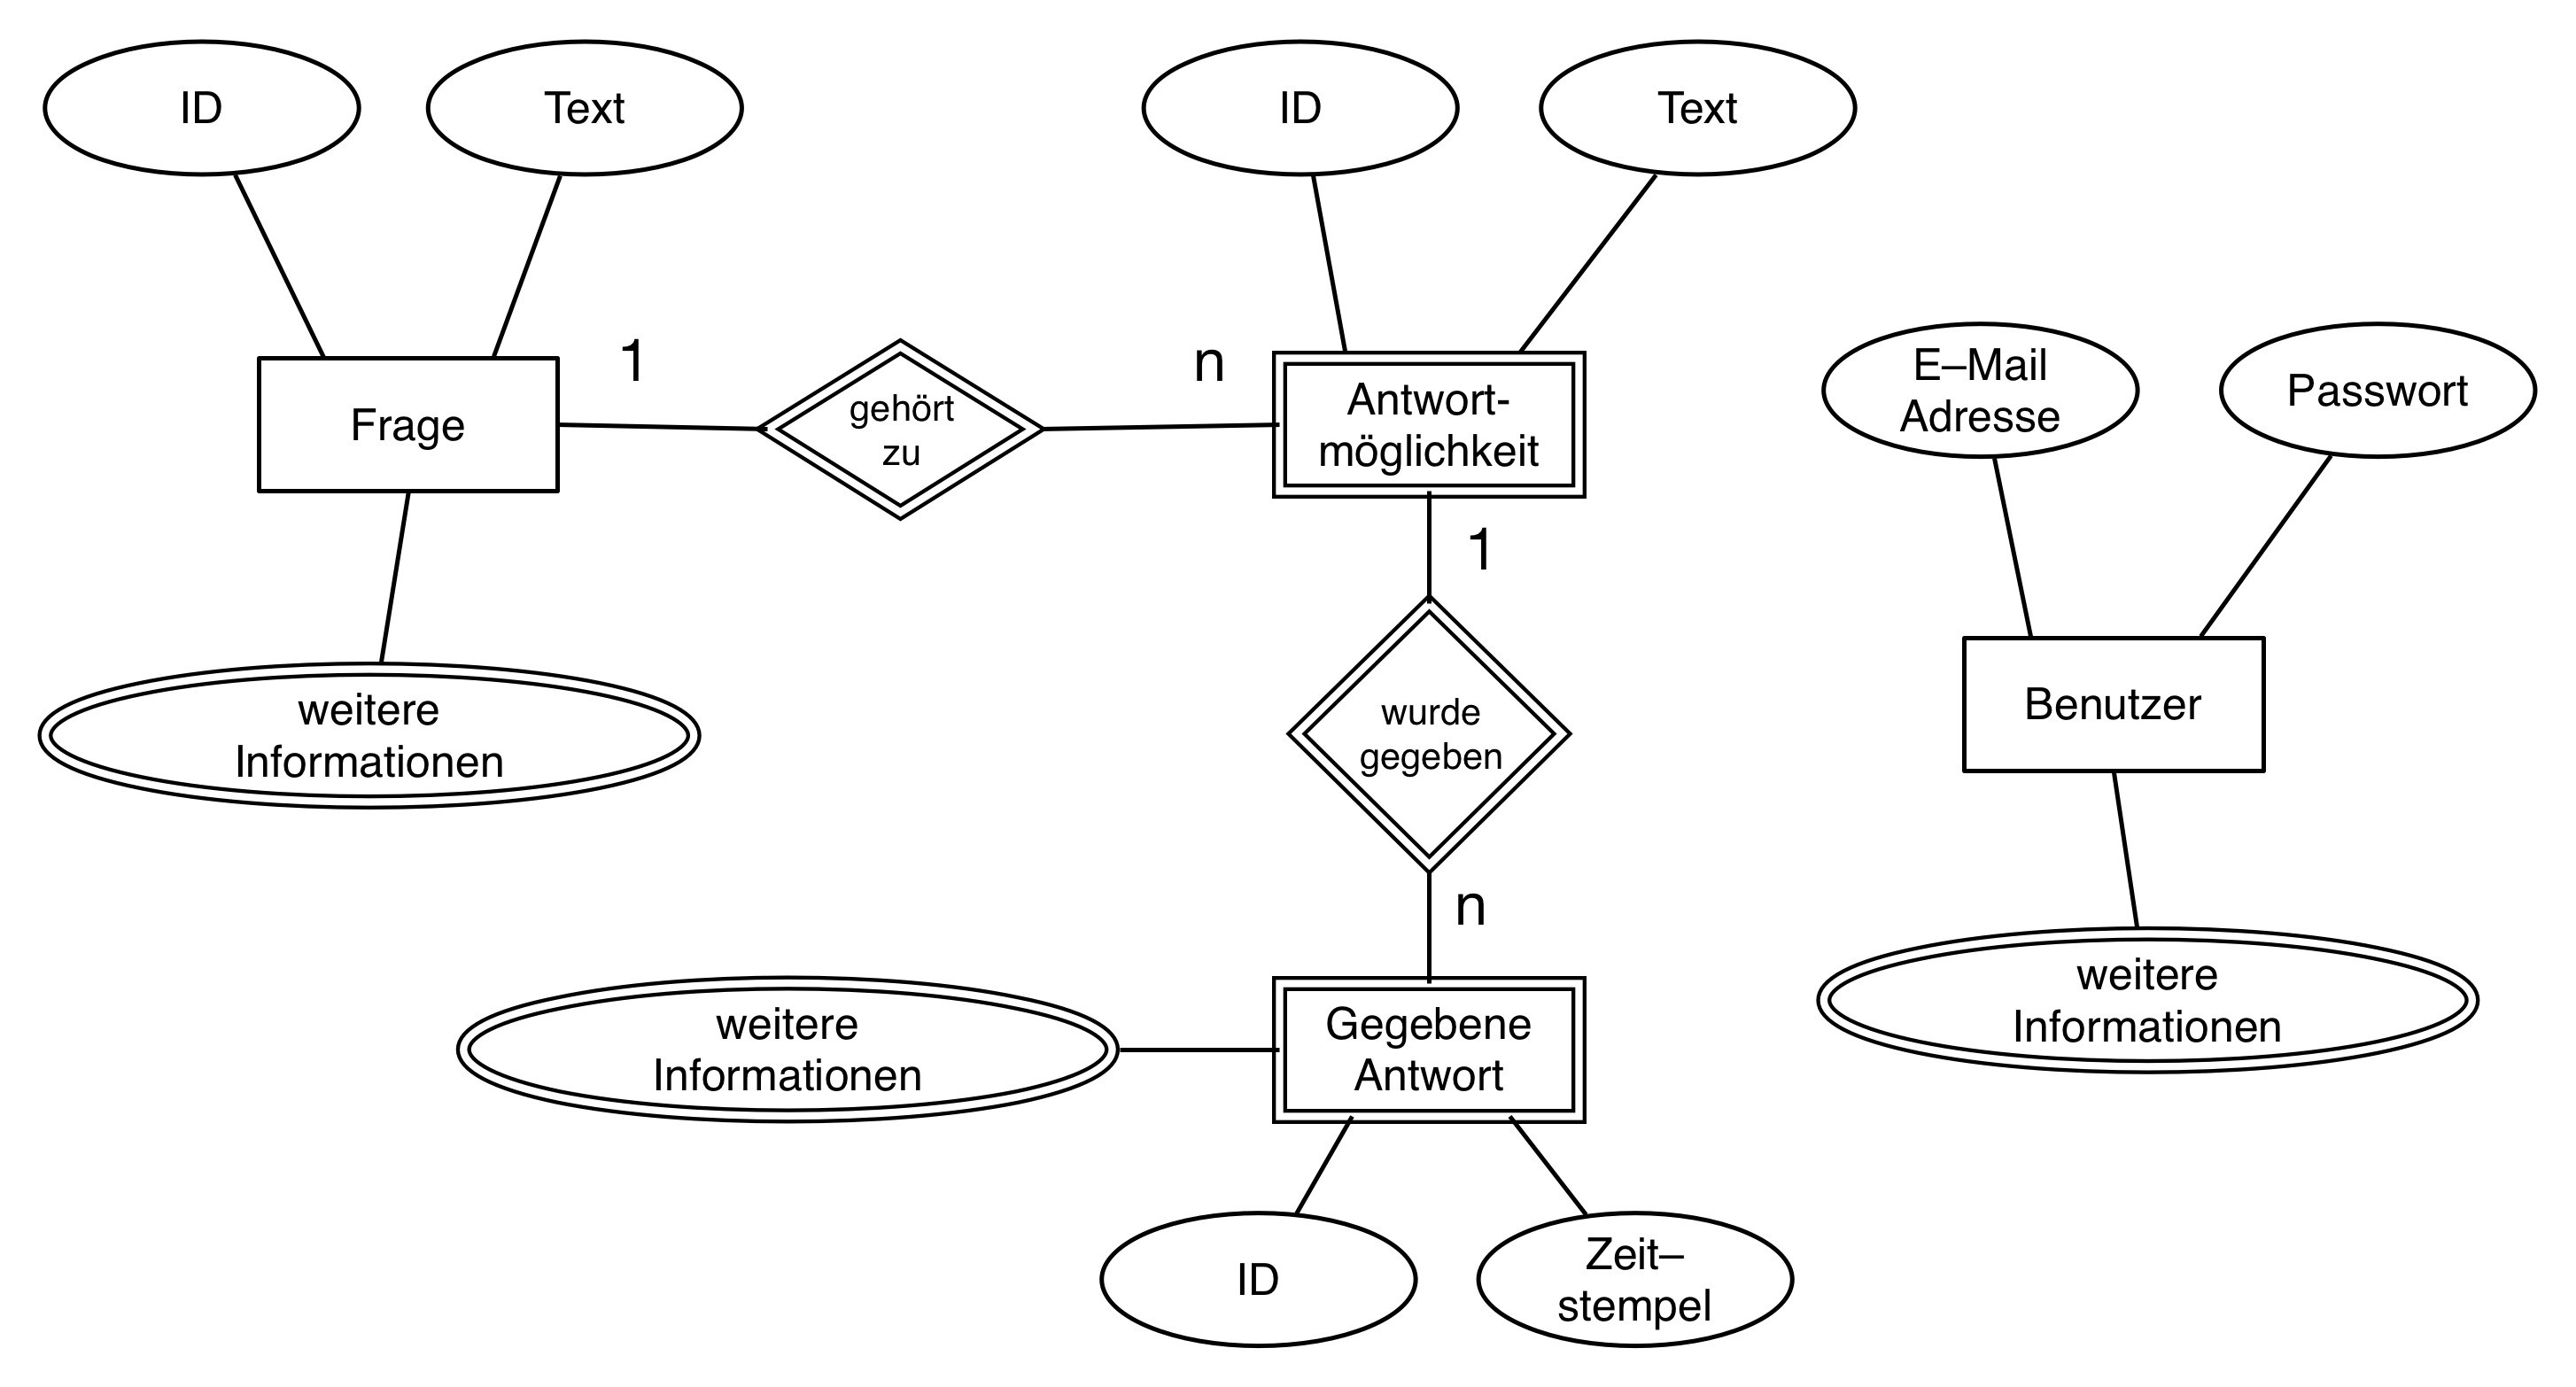
\includegraphics[width=\textwidth]{ERD.jpg}
\caption{Entity Relationship Diagram}
\end{center}
\label{fig:erd}
\end{figure}

Die als zsammengesetzte Attribute dargestellten „weiteren Informationen“ sind Attribute der jeweiligen Entitäten, die für die gestellten Anforderungen nicht notwendig sind, jedoch im Produktivbetrieb großen Zusatznutzen bieten könnten. So wäre es möglich die gegebenen Antworten durch die Speicherung der IP--Adresse, Browser--Fingerprinting\footnote{Die Identifikation eines speziellen Nutzers durch Konfigurationsdetails des Webbrowsers, Bildschirmgröße, Betriebssystemversion, etc. Siehe auch \url{https://panopticlick.eff.org/}} oder andere Techniken genauer zu identifizieren und somit einem bestimmten Nutzer zuzuordnen. Hierbei sind dann die jeweiligen Datenschutzbestimmungen zu beachten.

Die Datensätze der Entity „Frage“ könnten Zeitangaben enthalten, die festlegen wann bzw. wie lange eine Frage auf der Website angezeigt wird. Die Antwortmöglichkeiten könnten durch entsprechende Angaben zur Sortierreihenfolge geordnet werden.

\subsection{Logisches Datenbankschema: Relationales Datenmodell}

Aufgrund des in Abbildung \ref{fig:erd} auf Seite \pageref{fig:erd} dargestelten Modell ergibt sich die in Abbildung \ref{fig:relmod} dargestellten Relationen. Dieses Modell entspricht der 3. Normalform\footnote{Kriterien laut \cite{dao101}, Kapitel 3.4}.

\begin{figure}[H]
\begin{center}
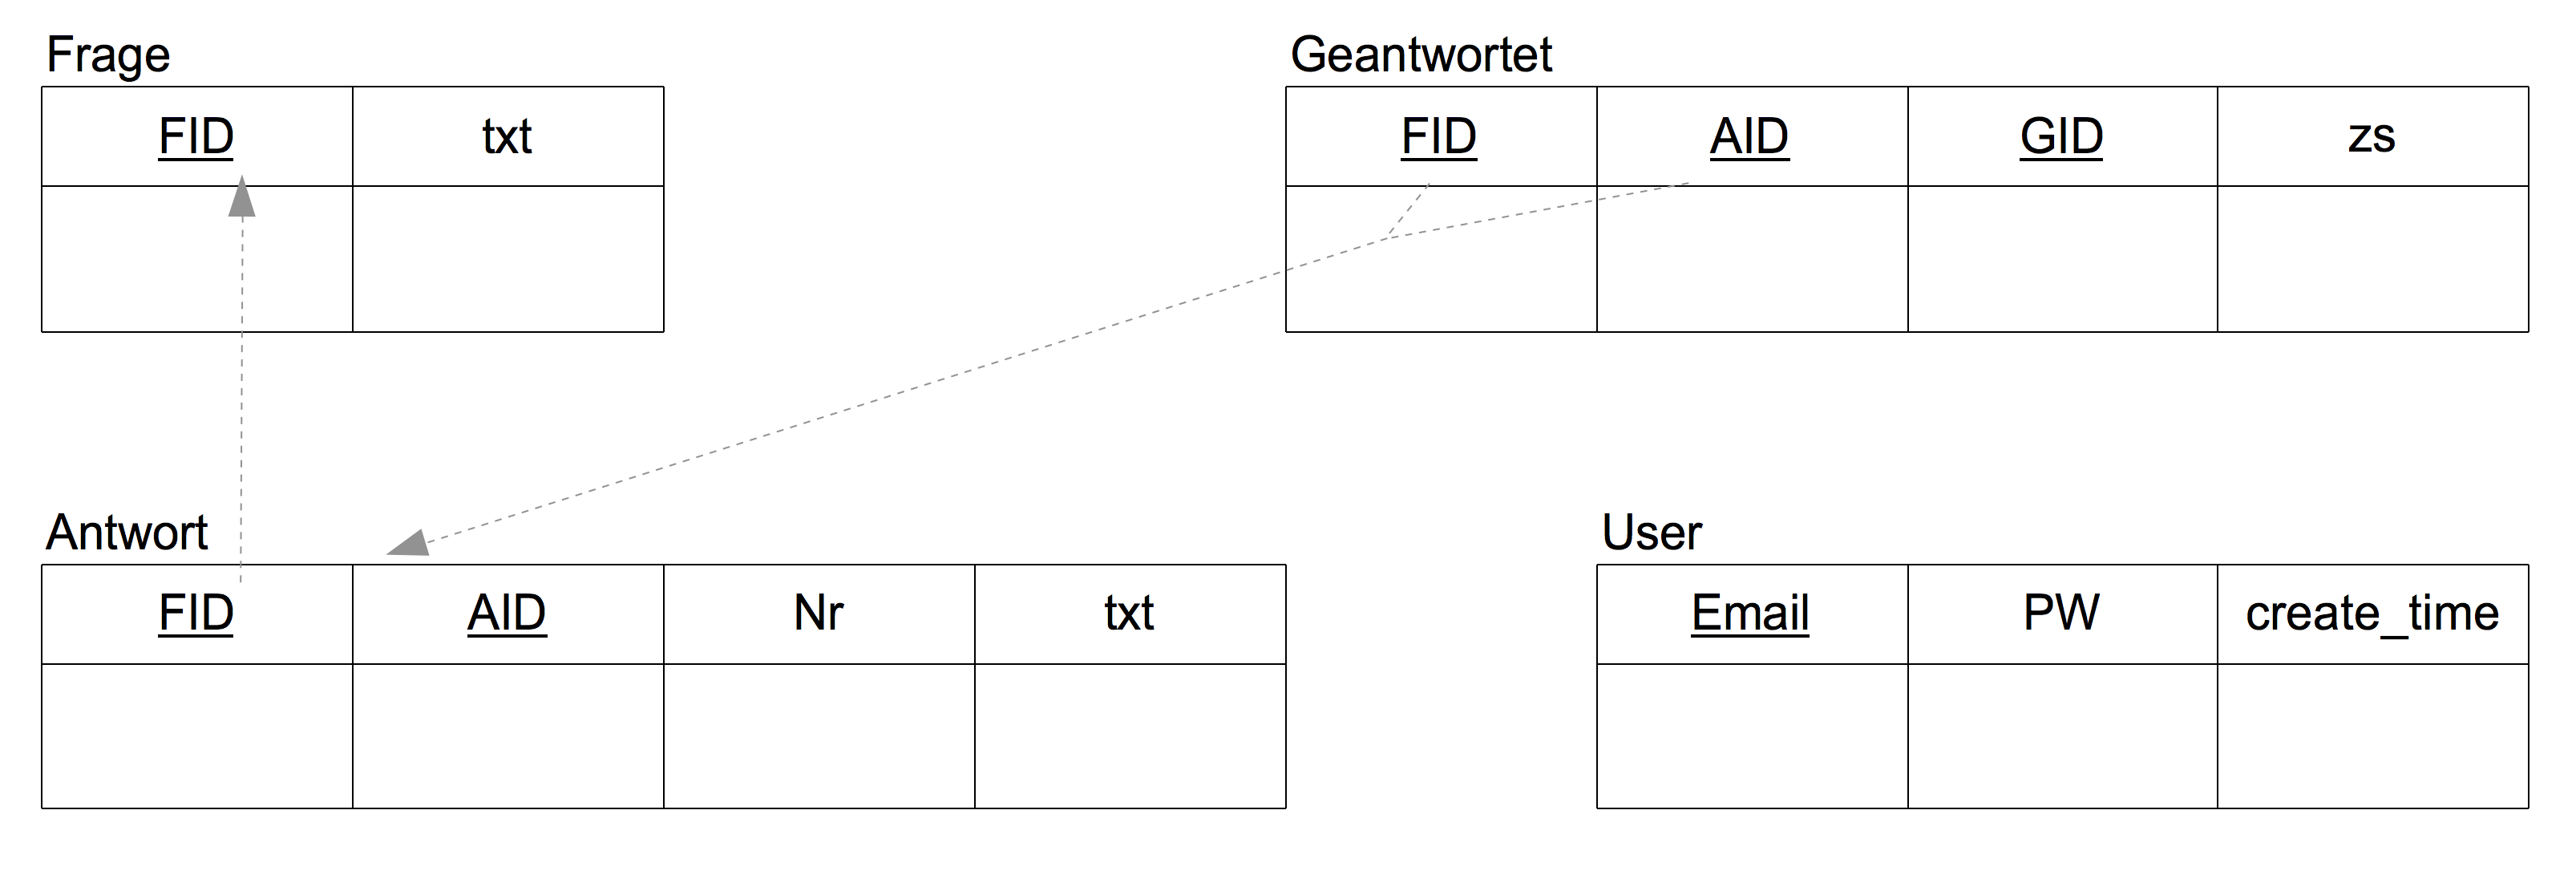
\includegraphics[width=\textwidth]{relmod.jpg}
\caption{Relationales Modell}
\end{center}
\label{fig:relmod}
\end{figure}

\subsection{Umsetzung in SQL}

\subsubsection{Tabelle: user --- Benutzerverwaltung}
\begin{figure}[H]
\begin{minted}[bgcolor=bg]{sql}
CREATE TABLE user (
  email VARCHAR(255) NOT NULL,
  pw CHAR(32) NOT NULL,
  create_time TIMESTAMP DEFAULT CURRENT_TIMESTAMP,
  PRIMARY KEY (`email`));
\end{minted}
\caption{SQL: CREATE TABLE user}
\label{sql:tbluser}
\end{figure}

Als Benutzername und auch als Primärschlüssel wird die E--Mail Adresse des Administrators genutzt. Da diese den Nutzer eindeutig identifiziert wird auf einen seperaten Nutzernamen und auch auf eine generierte ID als Primärschlüssel verzichtet.

Das Passwort sollte nicht im Klartext in der Datenbank gespeichert werden. Ein \code{salted hash}\footnote{Also der Hashwert des Passworts, welches zuvor mit Applikationsspezifischen Zusatzdaten ergänzt wurde} schützt hier das Passwort vor dem Ausspähen durch den Administrator selbst\footnote{Spätestens seit dem Datenklau bei Vodafone\footnote{\cite{vodafone}} eine dokumentierte Gefahr} oder durch Angreifer.\\
Die hier reservierten 32 Byte sind für den in der MySQL--Dokumentation\footnote{\cite{mysql:md5}} emphohlenen MD5-Hash ausreichend. Da die entsprechende PHP--Dokumentation\footnote{\cite{php:md5}} hier allerdings eine genau entgegengesetzte Empfehlung gibt, ist dieser Sicherheitsaspekt für ein Produktivsystem nochmals genauer zu prüfen.

\subsubsection{Tabelle: frage --- Fragestellungen}
\begin{figure}[H]
\begin{minted}[bgcolor=bg]{sql}
CREATE TABLE frage (
  fid INT NOT NULL AUTO_INCREMENT,
  txt VARCHAR(1024) NOT NULL,
  CONSTRAINT pk_frage PRIMARY KEY (`fid`));
\end{minted}
\caption{SQL: CREATE TABLE frage}
\label{sql:tblfrage}
\end{figure}

In der Tabelle „Frage“ wird lediglich der Text der Frage sowie die eindeutige Frage--ID gespeichert. Letztere dient als Primärschlüssel.

\subsubsection{Tabelle: antwort --- Antwortmöglichkeiten}
\begin{figure}[H]
\begin{minted}[bgcolor=bg]{sql}
CREATE TABLE antwort (
  fid INT NOT NULL, 
  aid INT NOT NULL AUTO_INCREMENT,
  nr  INT NULL,
  txt VARCHAR(1024) NOT NULL,
  CONSTRAINT pk_antwort PRIMARY KEY (fid, aid),
  CONSTRAINT fk_antwort_frage_fid FOREIGN KEY (fid) 
  REFERENCES frage(fid) 
  ON UPDATE CASCADE 
  ON DELETE CASCADE );
\end{minted}
\caption{SQL: CREATE TABLE antwort}
\label{sql:tblantwort}
\end{figure}

Aufgrund der Modellierung als schwache Entity setzt sich der Primärschlüssel der Tabelle „Antwort“ aus der Frage--ID sowie der Antwort--ID zusammen. Zusätzlich wird der Antworttext sowie eine frei zu vergebende Nummer gespeichert, welche für die Sortierreihenfolge bei der Anzeige genutzt werden kann.

Die Integritätsbedingung wird so definiert, dass beim Löschen einer Frage auch die zugehörigen Antwortmöglichkeiten gelöscht werden.

\subsubsection{Tabelle: geantwortet --- Gegebene Antworten}
\begin{figure}[H]
\begin{minted}[bgcolor=bg]{sql}
CREATE TABLE geantwortet (
  fid INT NOT NULL,
  aid INT NOT NULL,
  gid INT NOT NULL AUTO_INCREMENT,
  zs TIMESTAMP DEFAULT CURRENT_TIMESTAMP,
  CONSTRAINT pk_geantwortet PRIMARY KEY (fid, aid, gid),
  CONSTRAINT fk_geantwortet_antwort_aid FOREIGN KEY (fid, aid) 
  REFERENCES antwort(fid, aid) 
  ON UPDATE CASCADE 
  ON DELETE CASCADE );
\end{minted}
\caption{SQL: CREATE TABLE geantwortet}
\label{sql:tblgeantwortet}
\end{figure}

Für die Speicherung der gegebenen Antworten in der Tabelle „geantwortet“ genügt der aus Frage--ID, Antwort--ID und Geantwortet--ID zusammengesetzte Primärschlüssel. Zusätzlich wird noch der jeweilige Zeitstempel für spätere Auswertungen erfasst.

Auch hier stellt die Integritätsbedingung sicher, dass beim Wegfall der entsprechenden Antwortmöglichkeit keine undefinierten gegebene Antworten zurückbleiben.

\section{Klassenhierarchie}
\label{sec:klassen}
Der Zugriff auf die in der bislang beschriebenen Datenbank gespeicherten Daten erfolgt über die folgende  Klassenhierarchie:

\begin{figure}[H]
\begin{center}
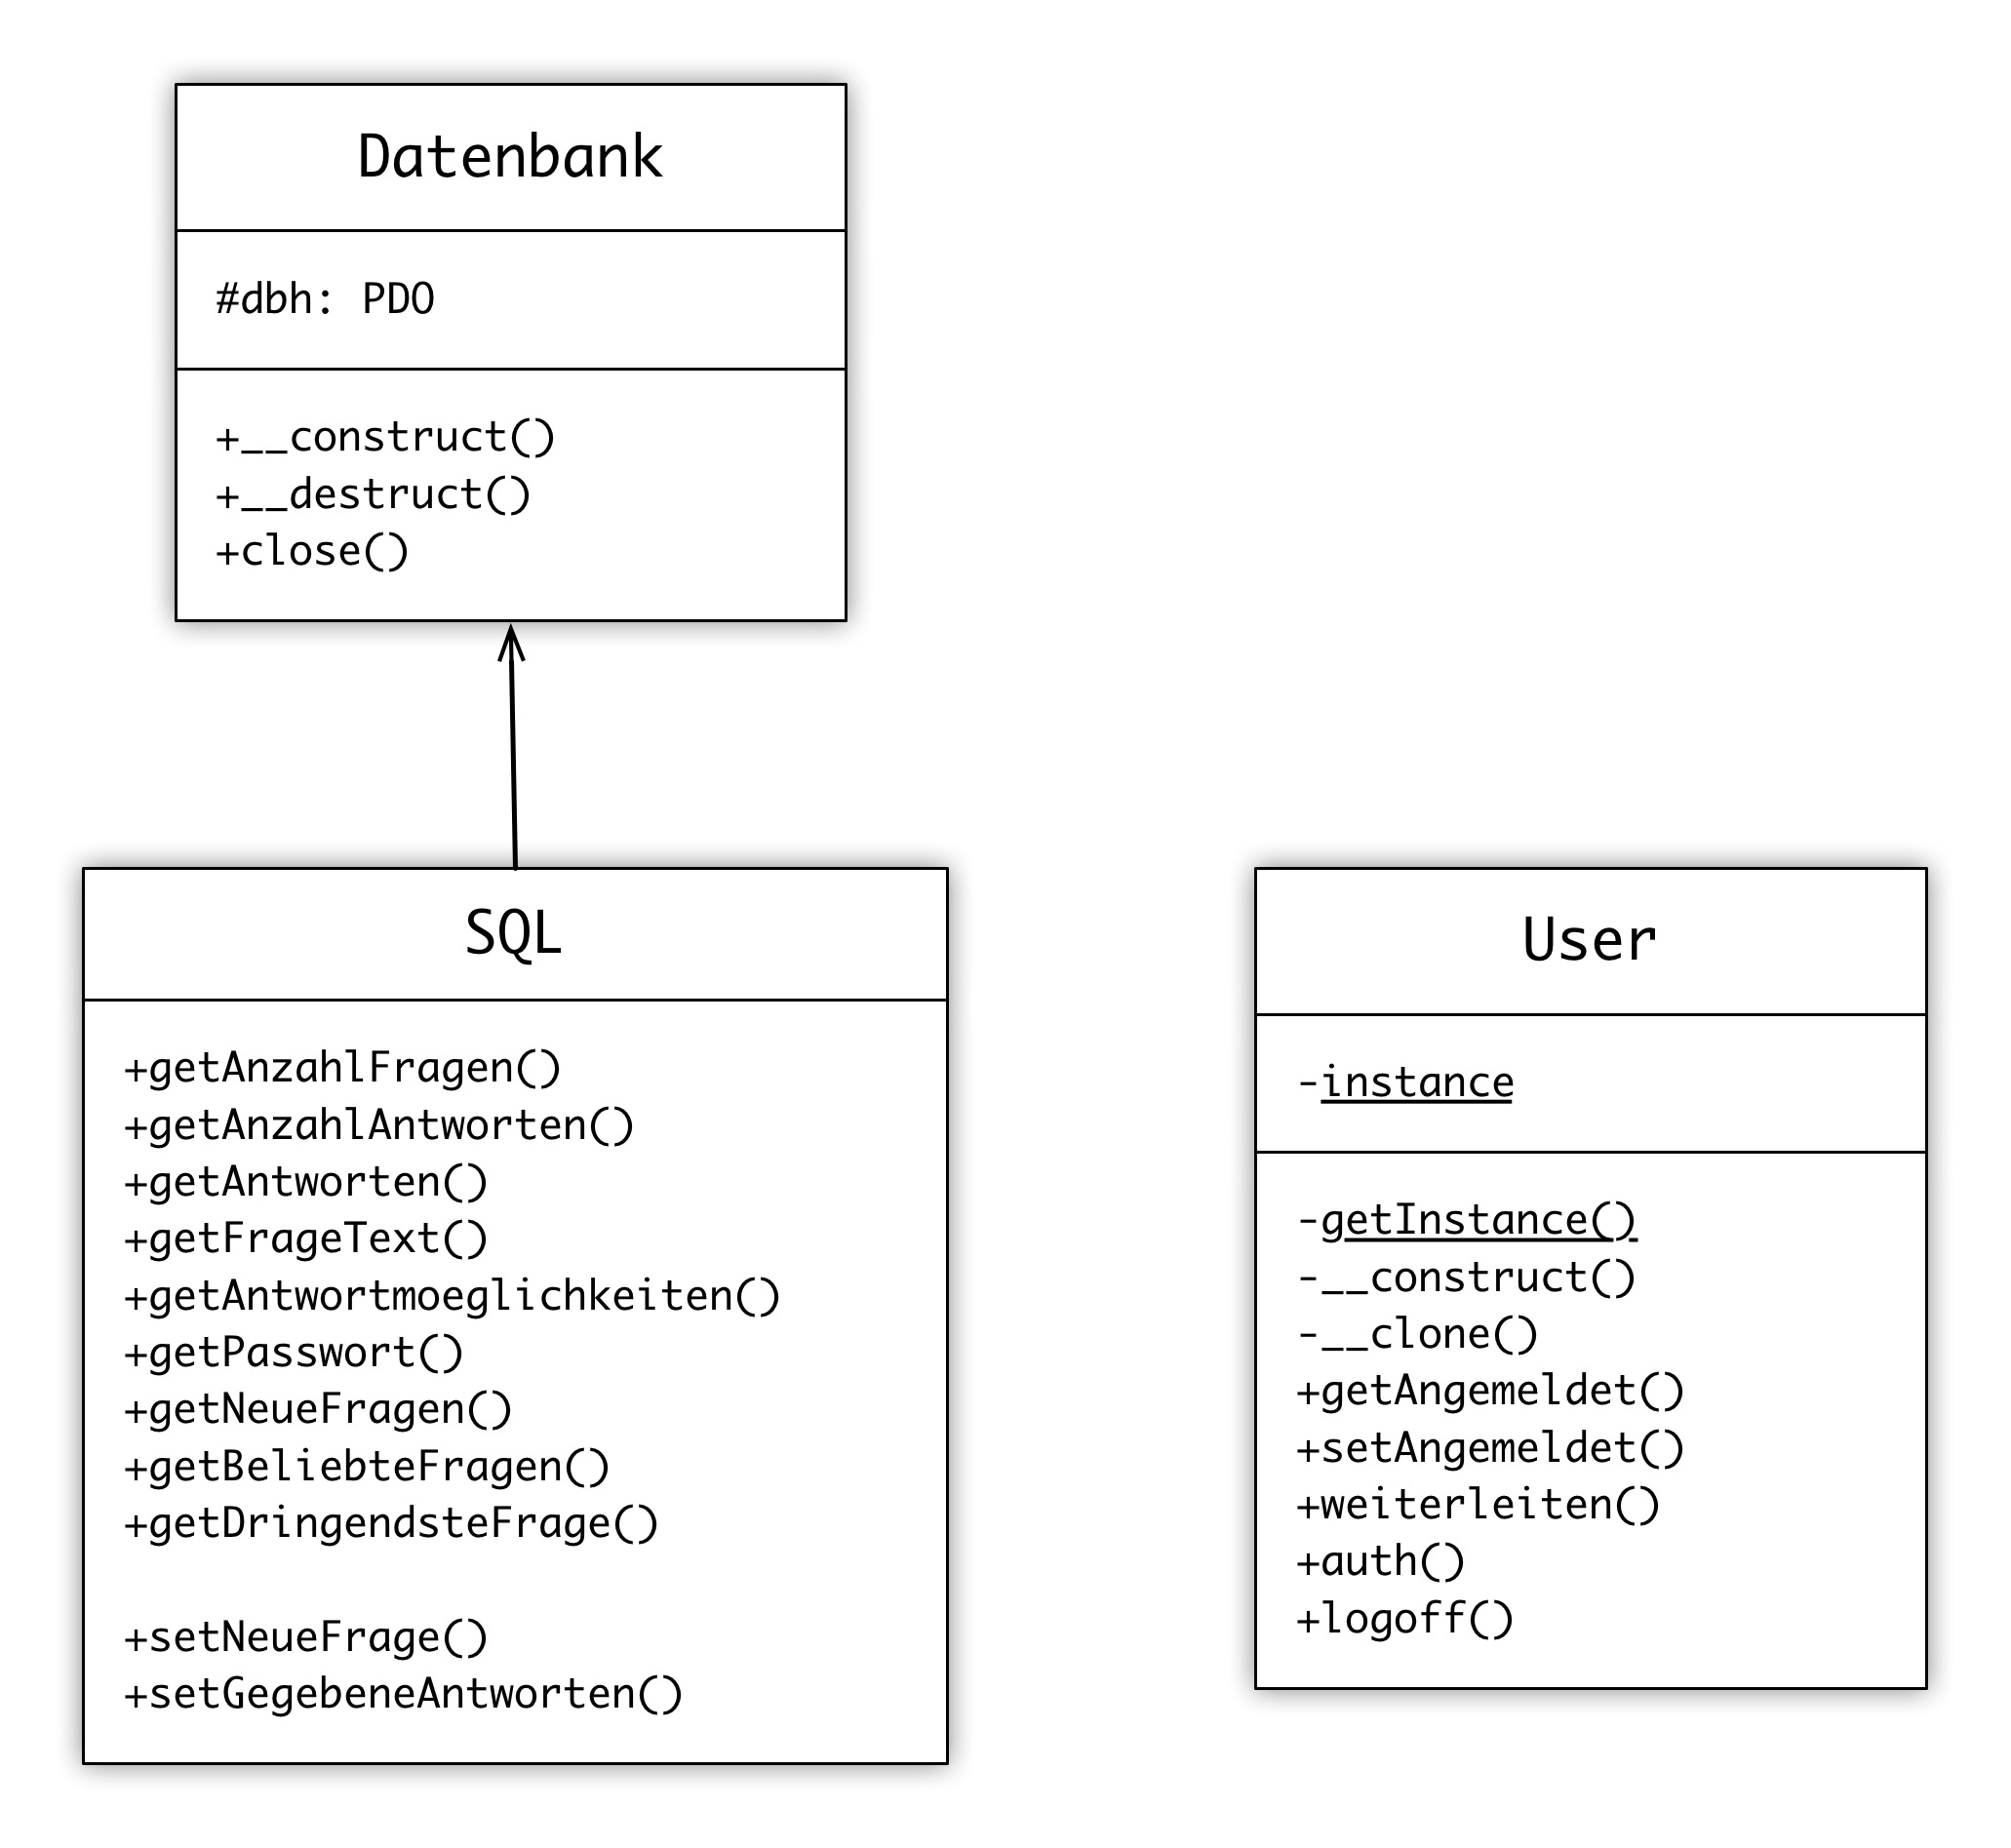
\includegraphics[width=\textwidth]{UML.jpg}
\caption{UML--Klassendiagramm}
\label{fig:uml}
\end{center}
\end{figure}

Die Implementation der Klassen ist im beigefügten Quelltext in den Dateien \code{.../class/Datenbank.php}, \code{.../class/SQL.php} und \code{.../class/User.php} zu betrachten. Auch die Klasse „User“ nutzt für den Datenbankzugriff die Klasse \code{SQL}. Dies geschieht allerdings nur innerhalb der Methode \code{auth()} über eine lokale Variable und ist daher im UML--Diagramm nicht zu erkennen.

\subsection{Klasse: Datenbank --- Low--Level Zugriff}

Die Klasse \code{Datenbank} stellt die unterste Ebene des Datenzugriffs der Anwendung dar. Aufgrund der von PHP zur Verfügung gestellten PDO--Klasse greift jedoch auch diese Klasse nicht direkt auf die Datenbank  zu. Das PDO--Objekt ist als Attibut in der Klasse vorhanden. Die für den Zugriff notwendigen Angaben werden im Konstruktor aus der Konfigurationsdatei \code{.../includes/dbconf.ini} gelesen und anschließend wird die Verbindung zur Datenbank hergestellt. 

Die Datenbankverbindung bleibt so lange bestehen wie die Instanz existiert. Ein Objekt mit geschlossener Datenbankverbindung würde die Notwendigkeit von zusätzlichen Fehlerprüfungen bzw. der erneuten Herstellung der Verbindung mit sich bringen. Um hierauf ausdrücklich hinzuweisen ist die Methode \code{close()} ohne Funktion definiert.
 
\subsection{Klasse: SQL --- High--Level Zugriff}

In der Klasse \code{SQL} werden die SQL--Abfragen gekapselt. Der aufrufende PHP--Code benötigt keinerlei Wissen über die zugrunde liegende Datenbank. Es müssen lediglich die Get-- und Set--Methoden eines Objektes vom Typ SQL aufgerufen werden. Innerhalb dieser Methoden werden dann die SQL--Abfragen mit Hilfe des geerbten PDO--Objekts vorbereitet und dann mit den geforderten Parametern aufgerufen. Die Ergebnisse werden dann als einzelner Wert oder als Objekt mit mehreren Werten bzw. Array zurückgegeben. Hierbei wird die jeweils geeignete Form gewählt.

Zum Speichern von neuen Fragen und Antwortmöglichkeiten bzw. von gegebenen Antworten werden diese an die entsprechenden Set--Methoden übergeben. Hierin werden die zum Abspeichern benötigten SQL-INSERTs in eine Trans\-aktion verpackt. Somit ist auch bei gleichzeitigem Zugriff mehrerer Nutzer oder im Fehlerfall ein konsistenter Zustand des Datenbestandes gesichert.

Durch die Reduzierung der Aufrufe auf die passenden Get-- und Set--Methoden wird in der SQL-Klasse das Fassaden-Entwurfsmuster realisiert. Der aufrufende Code benötigt keinerlei Informationen über die Datenstruktur, die Datenbank oder Transaktionen. Änderungen an diesen technischen Details wirken sich lediglich auf die SQL--Klasse aus. Solange diese laut Spezifikation Werte entgegennimmt und zurückliefert, muss kein weiterer Programmcode geändert werden.

\subsubsection{Speichern von neuen Fragen und Antwortmöglichkeiten}
\label{sec:speichern}
In der Methode \code{setNeueFrage()} werden neue Fragen und die zugehörigen Antwortmöglichkeiten in der Datenbank abgespeichert. Hierzu werden die entsprechenden Texte in den Parametern \code{\$fragetext} und \code{\$antworten} übergeben. Bei Letzterem handelt es sich um ein Array, da es pro Frage mehrere Antwortmöglichkeiten gibt.

Das Datenbankschema verlangt es, dass zu jeder Antwortmöglichkeit die ID der zugehörigen Frage gespeichert wird. Somit wird zunächst die Frage in die Datenbank eingefügt. Die automatisch generierte ID kann dann mit der PDO--Methode \code{lastInsertId()} ausgelesen werden. Anschließend werden die Antwortmöglichkeiten in einer \code{foreach}--Schleife in die Datenbank eingefügt.

Dieser Vorgang besteht somit aus vielen einzelnen Schritten. Fehlermöglichkeiten bestehen im PHP--Code selbst, sowie beim Zugriff auf die Datenbank. An jeder Stelle sind Unterbrechungen durch weitere Instanzen der Anwendung möglich, was im schlimmsten Fall zu einer inkorrekten Frage--ID führen könnte. Es ist sicherzustellen, dass entweder die gesamte Kombination von Frage mit allen zugehörigen Antwortmöglichkeiten gespeichert wird oder das Speichern gar nicht statt findet und mit einer entsprechenden Fehlermeldung abbricht. Im Fehlerfall darf keine Frage ohne den kompletten Antwortsatz in der Datenbank sein. 

Daher wird der gesamte Vorgang in einer SQL--Transaktion eingebettet und im Fehlerfall werden schon getätigte Änderungen mit einem Rollback zurückgenommen. Somit ist Konsistenz der Datenbank zu jedem Zeitpunkt sichergestellt.

\subsection{Klasse: User --- Benutzerverwaltung}
\label{sec:user}
Die Benutzerverwaltung nutzt das Singleton--Entwurfsmuster. Dieses wird durch die folgenden Maßnahmen implementiert: Die private Deklaration des Konstruktors sowie der \code{clone()} Methode wird die direkte Instanziierung der Klasse unterbunden. Eine Referenz auf die Instanz wird in der ebenfalls privaten statischen Variable \code{ \$instance } gespeichert und über die öffentliche Funktion \code{getInstance()} bekannt gemacht.

Die Funktion \code{auth()} erwartet als Parameter den Benutzernamen und das Passwort sowie optional eine URL, zu der im Falle der erfolgreichen Authentifizierung umgeleitet werden soll. Der Datenbankzugriff erfolgt über eine lokale Instanz der Klasse SQL. Stimmen die Anmeldedetails mit den in der Datenbank gespeicherten überein, werden in der von PHP zur Verfügung gestellten \code{\$\_SESSION}--Variable das Feld „angemeldet“ mit \code{TRUE} und das Feld \code{benutzer} mit dem Benutzernamen gefüllt. Stimmen die Anmeldedaten nicht mit den gespeicherten Werten überein, so erhält das Feld „angemeldet“ den Wert \code{FALSE}.

Die Funktion \code{logoff()} meldet den momentan angemeldeten Nutzer ab, in dem sie die Session-Variable zerstört und damit auch die Felder \code{angemeldet} und \code{benutzer} löscht.

Die Funktion \code{setAngemeldet()} ist eine private Hilfsmethode, mit der das Feld \code{angemeldet} der \code{\$\_SESSION}--Variable gesetzt werden kann. Da sie aus der Methode \code{getInstance()} heraus aufgerufen wird, ist sie wie diese auch statisch deklariert.

Die Funktion \code{getAngemeldet()} dient zur Anfrage des Anmeldestatus. Sie wird immer dann aus der Anwendung heraus aufgerufen, wenn der Seitenaufbau für angemeldete Benutzer anders sein soll, wie für nicht angemeldete. Am auffälligsten ist dies beim Aufruf der Seite zur Eingabe von neuen Fragen. Hier wird dem nicht angemeldeten Nutzer das Login--Formular angezeigt, während dem angemeldeten Nutzer die gewünschte Funktion direkt zur Verfügung steht.\\
Aber auch in Details können sich die Seiten unterscheiden: Die in der Seitenleiste angebotenen Links können schon entsprechend angepasst sein. Auf diese Weise werden dem Nutzer nur die Möglichkeiten gezeigt, die für ihn tatsächlich relevant sind. 

\section{Umsetzung in HTML \& PHP}

\subsection{Seitenstruktur}

Alle Seiten der Anwendung sind nach dem gleichen Muster aufgebaut. Sie werden von der Datei \code{index.php} erzeugt. Hier werden wie in Abbildung \ref{fig:struktur} auf Seite \pageref{fig:struktur} die Seitenelemente aus den verschiedenen Include--Dateien für den Kopfbereich, die Navigationsleiste am rechten Rand und dem Fußbereich zusammengesetzt\footnote{Darstellung vereinfacht}. Der eigentliche Funktionsbereich\footnote{Frage anzeigen, Antworten speichern und auswerten, anmelden, abmelden, Eingabemaske für neue Fragen sowie das Abspeichern der neuen Fragen} werden von den PHP--Dateien im Verzeichniss \code{.../pages/} übernommen.

\begin{figure}[h]
\begin{minted}[bgcolor=bg]{php}
<?php 
  include($_SERVER['DOCUMENT_ROOT'].'/includes/header.php'); 
?>
<div class="row">
 <div class="col-md-8">
  <?php 
    include($_SERVER['DOCUMENT_ROOT'].'/pages/'. $show . '.php'); 
  ?> 
 </div>
 <div class="col-md-4">
  <?php 
    include($_SERVER['DOCUMENT_ROOT'].'/includes/sidebar.php'); 
  ?>
 </div>	  
</div>
<?php 
  include($_SERVER['DOCUMENT_ROOT'].'/includes/footer.php'); 
?>
\end{minted}
\caption{HTML: Seitenstruktur und PHP--Includes}
\label{fig:struktur}
\end{figure}


Diese Seitenelemente und Programmteile werden in einer Struktur aus \code{DIV}--Elementen angeordnet, welche durch die CSS--Klassen des Bootstrap--Frameworks zu einem modernen, responsiven Layout ausgezeichnet werden. Der Anwendungsentwickler braucht sich somit nicht um die optimale Darstellung der HTML--Seiten auf Desktoprechnern, Tabletts oder Smartphones zu kümmern. Jede Bildschirmgröße erhält durch Bootstrap automatisch ein speziell abgestimmtes Layout.


\subsection{Layoutanpassungen mit CSS}

Die Gestaltung des Layouts mit „Cascading Stylesheets“ (kurz: CSS) ermöglicht es, das durch das Bootstrap--Framework vorgegebene Aussehen durch hinzufügen eines eigenen Stylesheets anzupassen.

So wurden bei der besprochenen Anwendung die Überschriften in der Seitenleiste individuell Farbig unterstrichen. Die Thematischen Blöcker werden hierzu in \code{DIV}--Blöcken mit den entsprechenden CSS--IDs eingeschlossen. Wie in Abbildung \ref{fig:seitenleiste} auf Seite \pageref{fig:seitenleiste} zu sehen, werden die Links beim berühren mit dem Mauszeiger in der gleichen Farbe dargestellt.

Bei der Darstellung der Auswertung werden die vom Benutzer selbst gegebenen Antworten durch Auszeichnung mit einer CSS-Klasse in fetter Schrift hervorgehoben. 

\begin{figure}[h]
\begin{center}
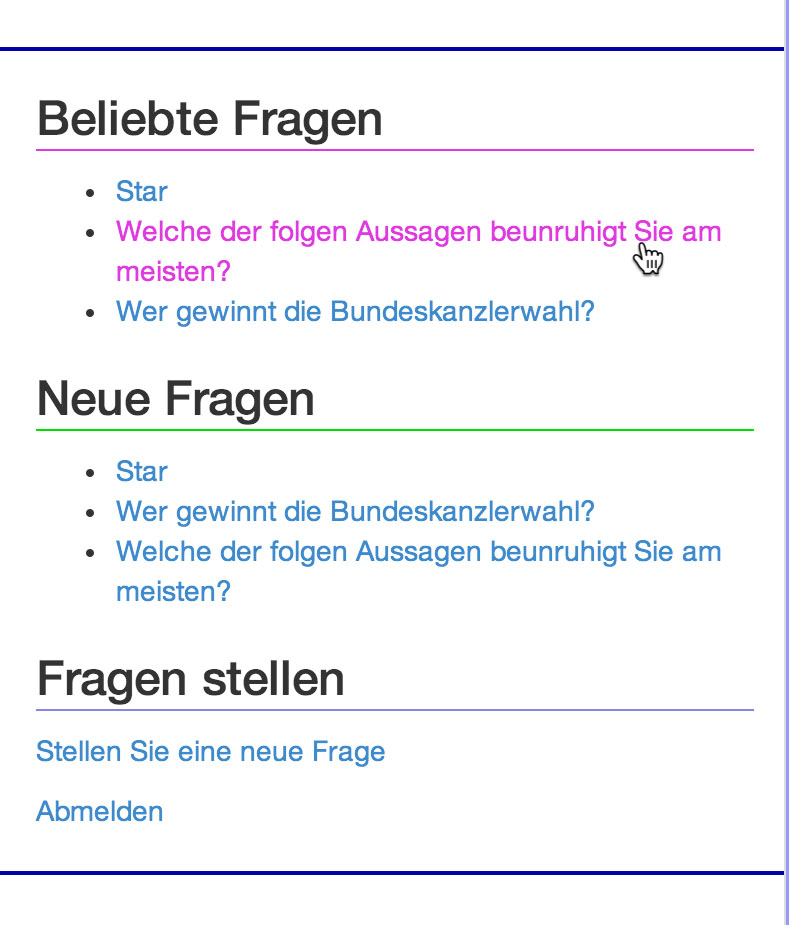
\includegraphics[width=\textwidth]{seitenleiste.jpg}
\caption{Unterstreichung und Link--Hervorhebung}
\end{center}
\label{fig:seitenleiste}
\end{figure}



\subsection{Mögliche Benutzerpfade durch die Anwendung}

Abbildung \ref{fig:zustaende} auf Seite \pageref{fig:zustaende}

\begin{figure}[h]
\begin{center}
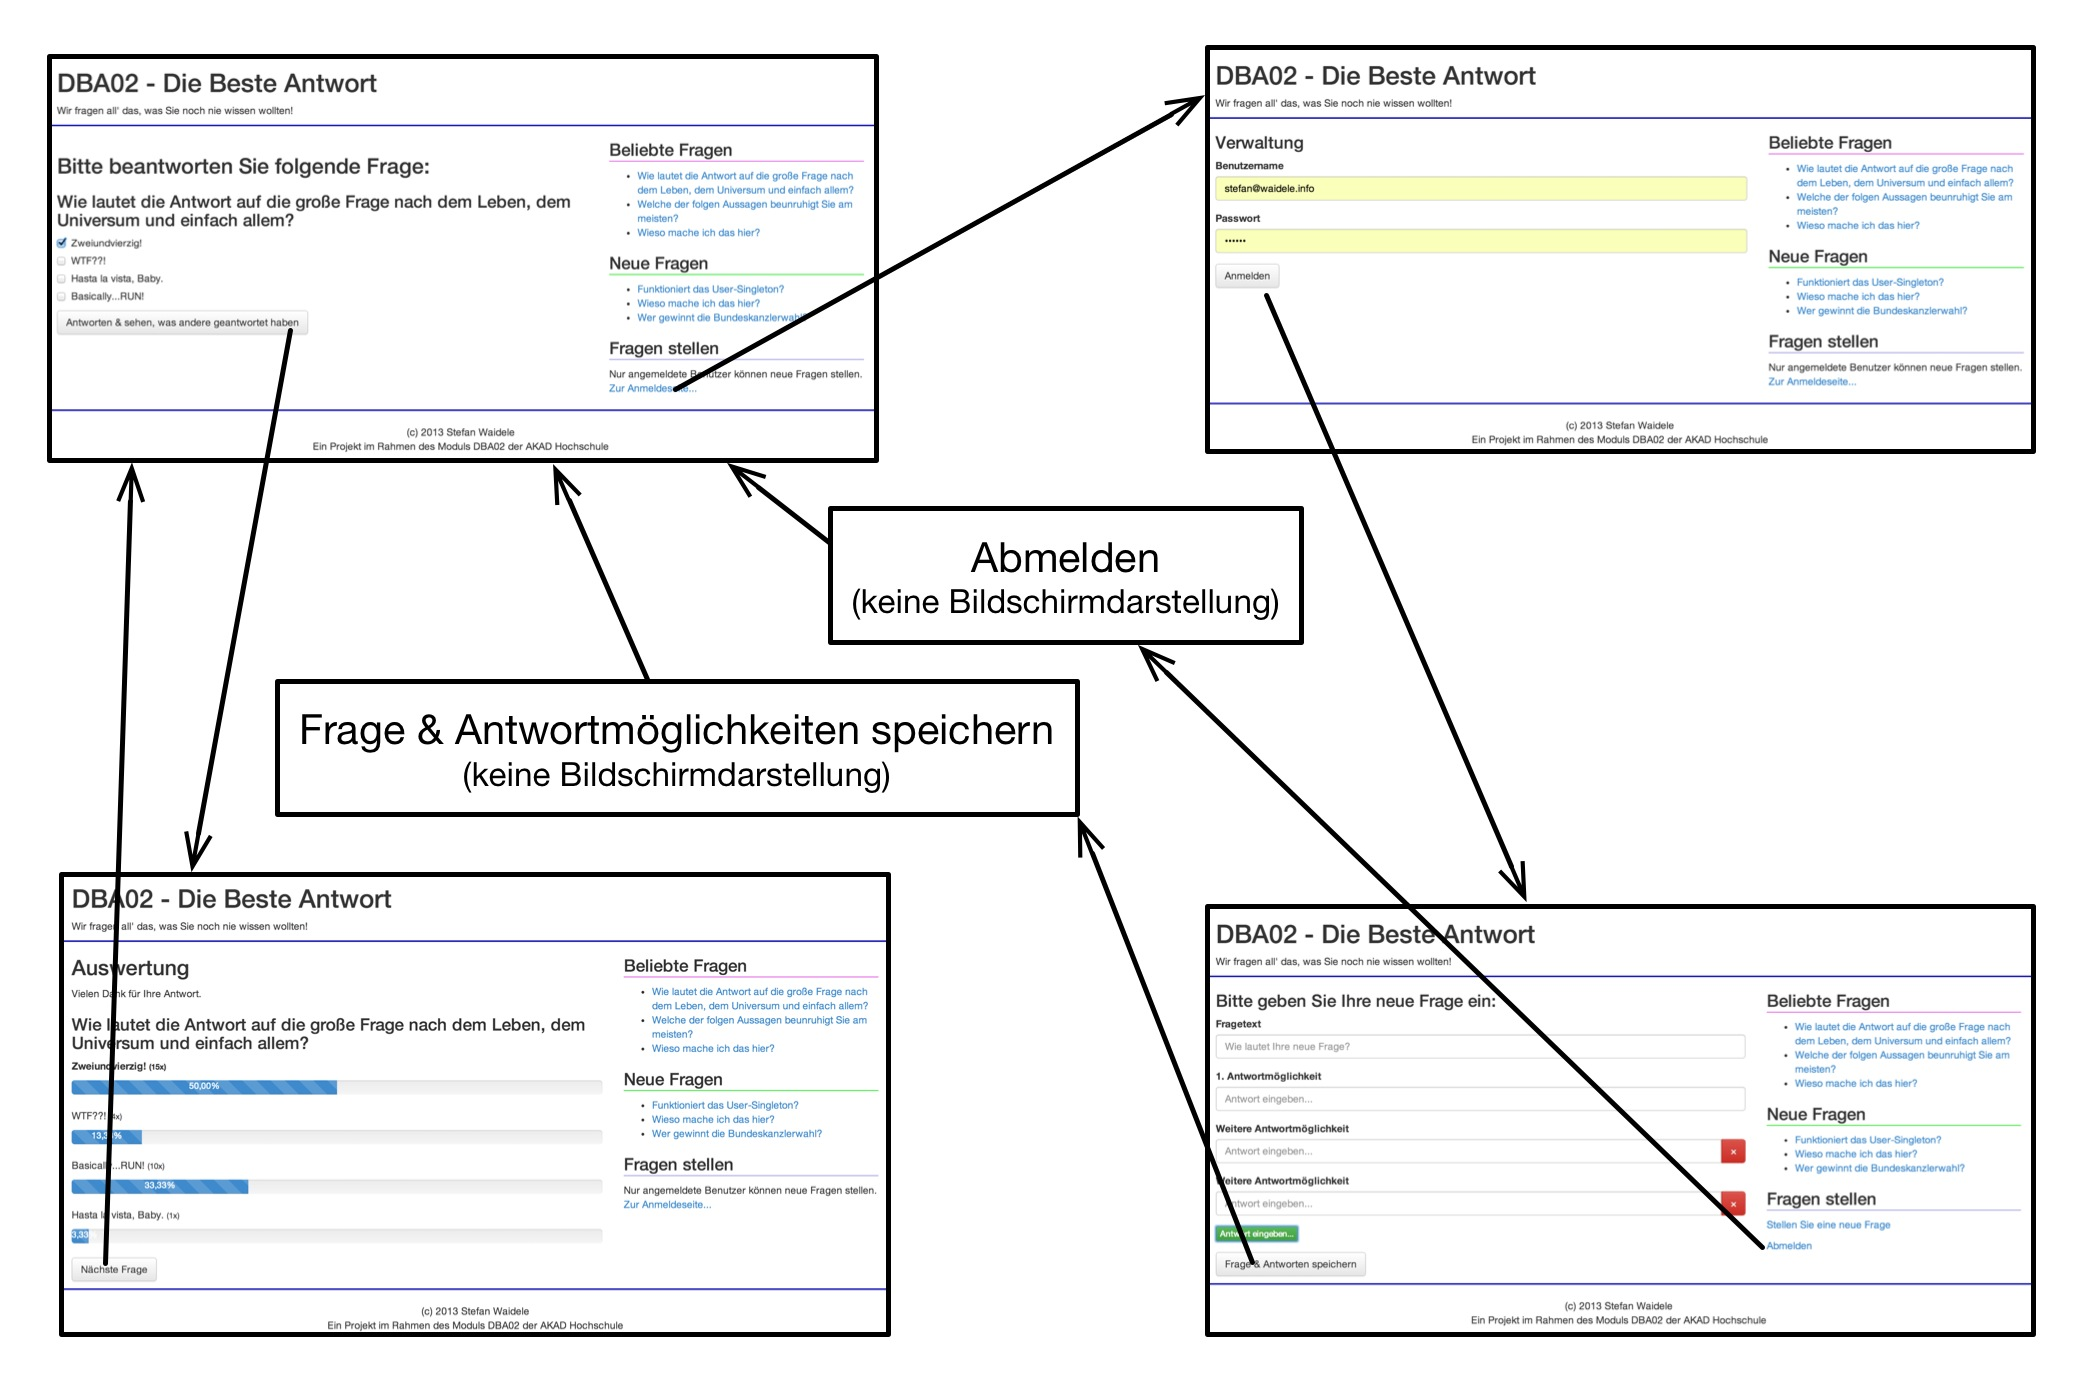
\includegraphics[width=\textwidth]{zustaende.jpg}
\caption{HTML--Seiten und Verlinkungen}
\end{center}
\label{fig:zustaende}
\end{figure}




\section{Bewertung}

\subsection{Zusammenfassung}
Lorem ipsum dolor sit amet, consetetur sadipscing elitr, sed diam nonumy eirmod tempor invidunt ut labore et dolore magna aliquyam erat, sed diam voluptua. At vero eos et accusam et justo duo dolores et ea rebum. Stet clita kasd gubergren, no sea takimata sanctus est Lorem ipsum dolor sit amet.

\subsection{kritische Würdigung}
Lorem ipsum dolor sit amet, consetetur sadipscing elitr, sed diam nonumy eirmod tempor invidunt ut labore et dolore magna aliquyam erat, sed diam voluptua. At vero eos et accusam et justo duo dolores et ea rebum. Stet clita kasd gubergren, no sea takimata sanctus est Lorem ipsum dolor sit amet.

\subsection{Ausblick}
Lorem ipsum dolor sit amet, consetetur sadipscing elitr, sed diam nonumy eirmod tempor invidunt ut labore et dolore magna aliquyam erat, sed diam voluptua. At vero eos et accusam et justo duo dolores et ea rebum. Stet clita kasd gubergren, no sea takimata sanctus est Lorem ipsum dolor sit amet.

\subsection{Erfolgsfaktoren}
Lorem ipsum dolor sit amet, consetetur sadipscing elitr, sed diam nonumy eirmod tempor invidunt ut labore et dolore magna aliquyam erat, sed diam voluptua. At vero eos et accusam et justo duo dolores et ea rebum. Stet clita kasd gubergren, no sea takimata sanctus est Lorem ipsum dolor sit amet.

\end{spacing}

\clearpage

% Literaturverzeichniss - Ab hier wieder Roemische Seitenzahlen
\pagestyle{plain}
\pagenumbering{roman}
\setcounter{page}{\theromanPagenumber}
\bibliographystyle{apalike}
\bibliography{literatur}
\onehalfspacing
\clearpage

\pagestyle{empty} 
\thispagestyle{empty}

\begin{center}
{\Large Eidesstattliche Erklärung}
\vspace*{4cm}\end{center}
\noindent
Ich versichere, dass ich das beiliegende Assignment selbstständig verfasst, keine anderen als die angegebenen Quellen und Hilfsmittel benutzt sowie alle wörtlich oder sinngemäß übernommenen Stellen in der Arbeit gekennzeichnet habe. 
\vspace{3cm}

\hspace{-0.8cm}
\rule[0.5ex]{6.5cm}{1pt}
\hspace{1.3cm}
\rule[0.5ex]{6.5cm}{1pt}
(Datum, Ort)
\hspace{6.3cm}(Unterschrift)

\clearpage

%Messbox zur Druckkontrolle:
\newcommand{\Messbox}[2]{% Parameters: #1=Breite, #2=Hoehe
\setlength{\unitlength}{1.0mm}%
\begin{picture}(#1,#2)%
\linethickness{0.05mm}%
\put(0,0){\dashbox{0.2}(#1,#2)%
{\parbox{#1mm}{%
\centering\footnotesize 
%{\bf MESSBOX}\\ 
Breite $ = #1 {\rm\ mm}$\\
H\"ohe $ = #2 {\rm\ mm}$
}}}\end{picture}
}

\begin{center}
\textbf{--- Druckgröße kontrollieren! ---}
\\
\Messbox{100}{50} % Angabe der Breite/Hoehe in mm
\\
\textbf{--- Diese Seite nach dem Druck entfernen! ---}
\end{center}


\end{document}

